\documentclass[14pt]{extarticle}
\usepackage[utf8]{inputenc}
\usepackage[a4paper, margin=1in]{geometry}
\usepackage{tikz}
\usepackage{color}
\usepackage{subfiles}
\usepackage[T1]{fontenc}
\usepackage{verbatim}
\usepackage{titlepic}
\usepackage{amssymb}
\usepackage{graphicx}
\usepackage{wrapfig}
\usepackage{caption}
\usepackage{subcaption}
\usepackage{listings}
\usepackage{minted}
\usepackage[section]{placeins}

\title{\Huge{\textcolor{blue}{TCP Reset Attack on Video Streaming}} \\ ~\\
        \LARGE{Report} \\ ~ \\ ~ \\ }
\author{Abdullah Al Ishtiaq \\
        \textbf{Student Id. : 1505080} \\ 
        Section: B ~~~~~ Group: 6}
\date{\today}


\begin{document}

\maketitle

\vspace{1cm}

\begin{figure}[h!]
\centering
    
\includegraphics[width = 0.25\textwidth]{Pictures/logoBUET.png}
\end{figure}
\begin{center}
\vspace{.5cm}

\Large{Department of Computer Science and Engineering \\
    Bangladesh University of Engineering and Technology \\
    (BUET) \\
    Dhaka - 1000 }

\end{center}

\newpage
%==================================================================

\tableofcontents

\vspace{3 cm}

\listoffigures
\newpage

%==================================================================

\section{Introduction}
    The Transmission Control Protocol (TCP) is a core protocol of the Internet Protocol Suite. It is one of the 2 main transport layer protocols which sit on top of the IP layer. TCP provides reliable, ordered and error-checked host-to-host communication services for applications. It is considered a stateless protocol suite because each client connection is newly made without considering whether a previous connection had been established or not. 
    
    Although TCP is widely used in major internet applications, it introduces a few vulnerabilities too. The most common of these vulnerabilities are: Denial of Service (DOS), Connection Hijacking, TCP Veto, TCP Reset attack etc.

\section{TCP Reset Attack on Video Streaming}
    TCP reset attack does not target the protocol's typical method of closing a connection which uses a 4-way handshake method. Rather it uses the protocol's special method of immediately terminating an unwanted, unexpected or erroneous connection. From the specifications of Transmission Control Protocol (TCP) given in RFC-0793 (September 1981) we quote, "Reset (RST) must be sent whenever a segment arrives which apparently is not intended for the current connection". It is an important property of TCP for ensuring robustness, but at the same time it has opened up a scope of exploitation. 
    
    In TCP reset attack on video streaming, an attacker forges a spoofed RST packet that pretends to be the one coming from the original video streaming server. As a result the victim immediately closes the TCP connection and goes to CLOSED state. In addition to that, upon receiving additional packets from the original server, the victim itself sends RST packet to the server terminating the connection at the remote end. In this way the attacker can successfully disrupt video streaming on its victim's machine.

\section{Strategy}
   
    The strategy of our attack can be described in 3 steps. Those are:
    \begin{enumerate}
      \item First we need to find out the IP address of either the victim machine or the video server. There can be quite a few machines connected to the same network and as long as we do not want to disrupt TCP connections on all of them, we need to know this information in particular prior to proceeding with our tool. Otherwise a port scanning mechanism would have sufficed. 
      \item Then we have to sniff packets in the network to discover the other IP address, the TCP port numbers and the correct sequence number. For this purpose, the tool will require additional feature of ARP Spoofing.
      \item Finally we forge a TCP packet with correct IP addresses, TCP Port numbers and sequence number and with RST bit set and send it to the victim machine.
    \end{enumerate}
    
    \label{sec:strategy}
    
    \textsl{Here one important aspect needs to be discussed. We can also perform the attack by sending forged RST packets to the video streaming server, but chances are that it will be self harmful as the server may block the attacker's IP address. So instead of doing so, we are going to send the forged packets to the victim machine.} 
    
    \textsl{Another important note is that we must send the packet with haste as the sequence number in the forged RST packet must be within victim's window to  be effective. Otherwise it will be discarded without any impact on the connection.}
  

\section{Timing Diagrams}
    Timing diagrams are really important in designing an attack tool as it gives us the insight about how the protocol actually works and how an attack can exploit its various vulnerabilities. For this reason, we have closely examined the specifications of the Transmission Control Protocol provided in RFC-0793 and accordingly drawn these timing diagrams with appropriate states.
    
    \subsection{Typical Timing Diagram}
        In Figure \ref{fig:TCP_Tim}, the timing diagram of typical communication for video streaming between the streaming server and victim is shown. At first the connection is established through a 3-way handshake. In the "ESTABLISHED" state the two parties can start exchanging messages which are represented in the figure as "ABC", "DEF", etc. The connection can finally be closed at the end of the communication by either of the parties and in both cases another 4-way handshake will occur. 
        
        \begin{figure}[!t]
        	\centering
        	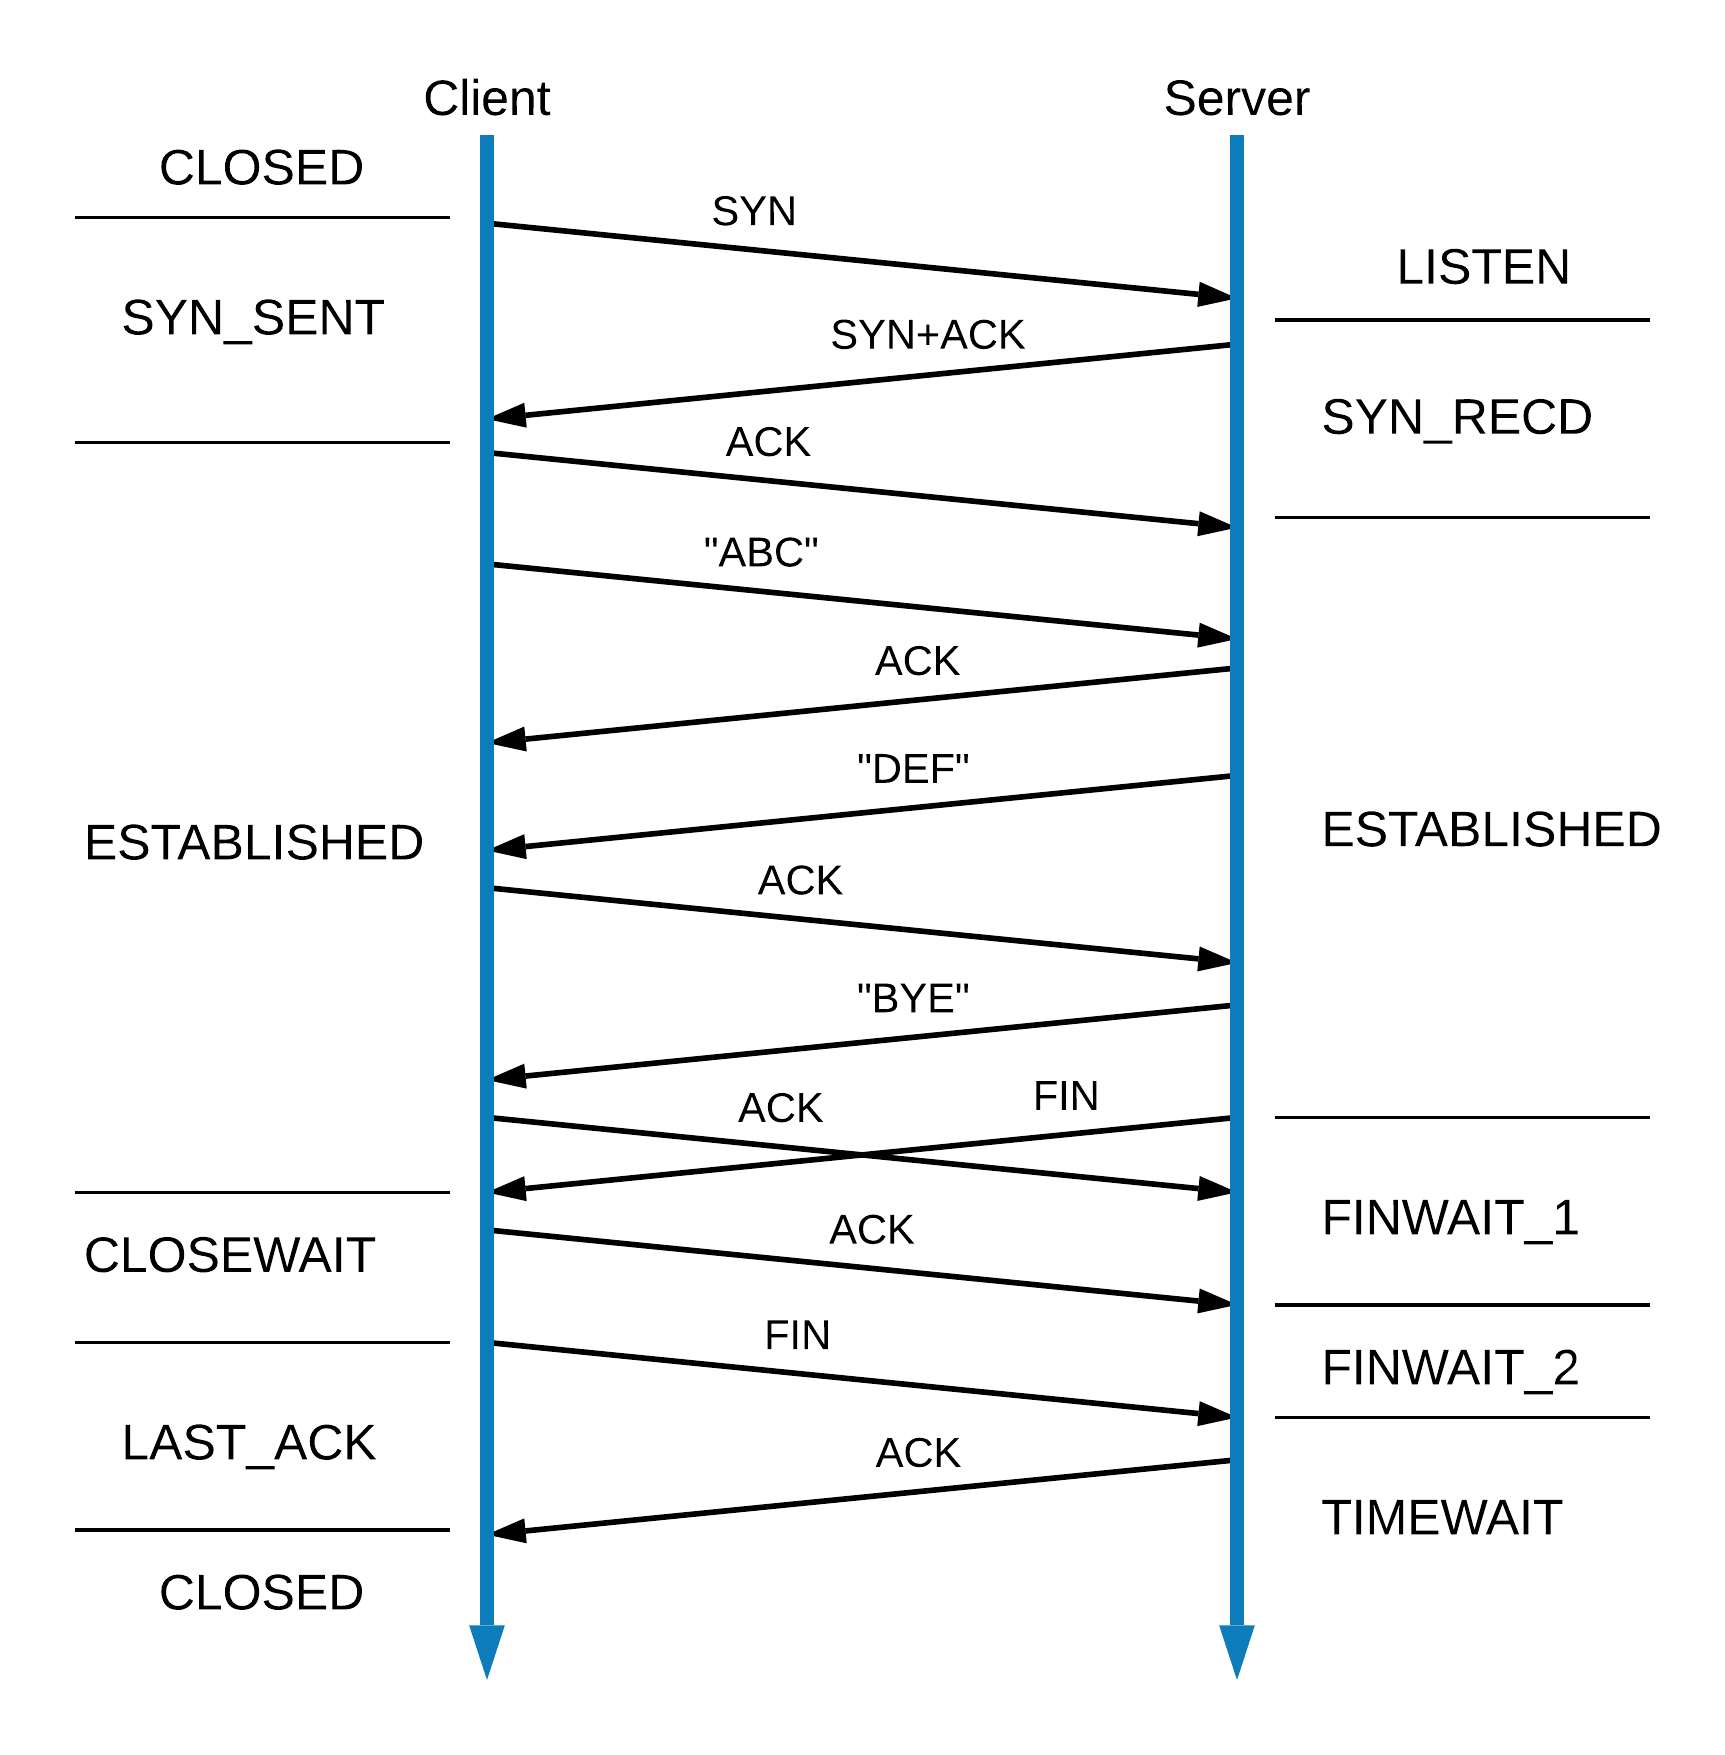
\includegraphics[width=.95\textwidth]{Pictures/Design/TCP_Timing_Diagram.png}
        	\caption{TCP Timing Diagram}
        	\label{fig:TCP_Tim}
        \end{figure}
    
    \newpage    
    \subsection{Attack Timing Diagram}
    
    We will perform the TCP reset attack by sending forged RST packet from the attacker machine. The timing diagram of the attack is shown in Figure \ref{fig:RST_Attack_Tim}. In this case the victim will assume the video server has unexpectedly terminated the "ESTABLISHED" TCP connection, and immediately close the connection. Upon receiving additional messages from the actual server it will send RST back and finally the server will also close the connection receiving the RST packet. \\ 
    
    \begin{figure}
    	\centering
    	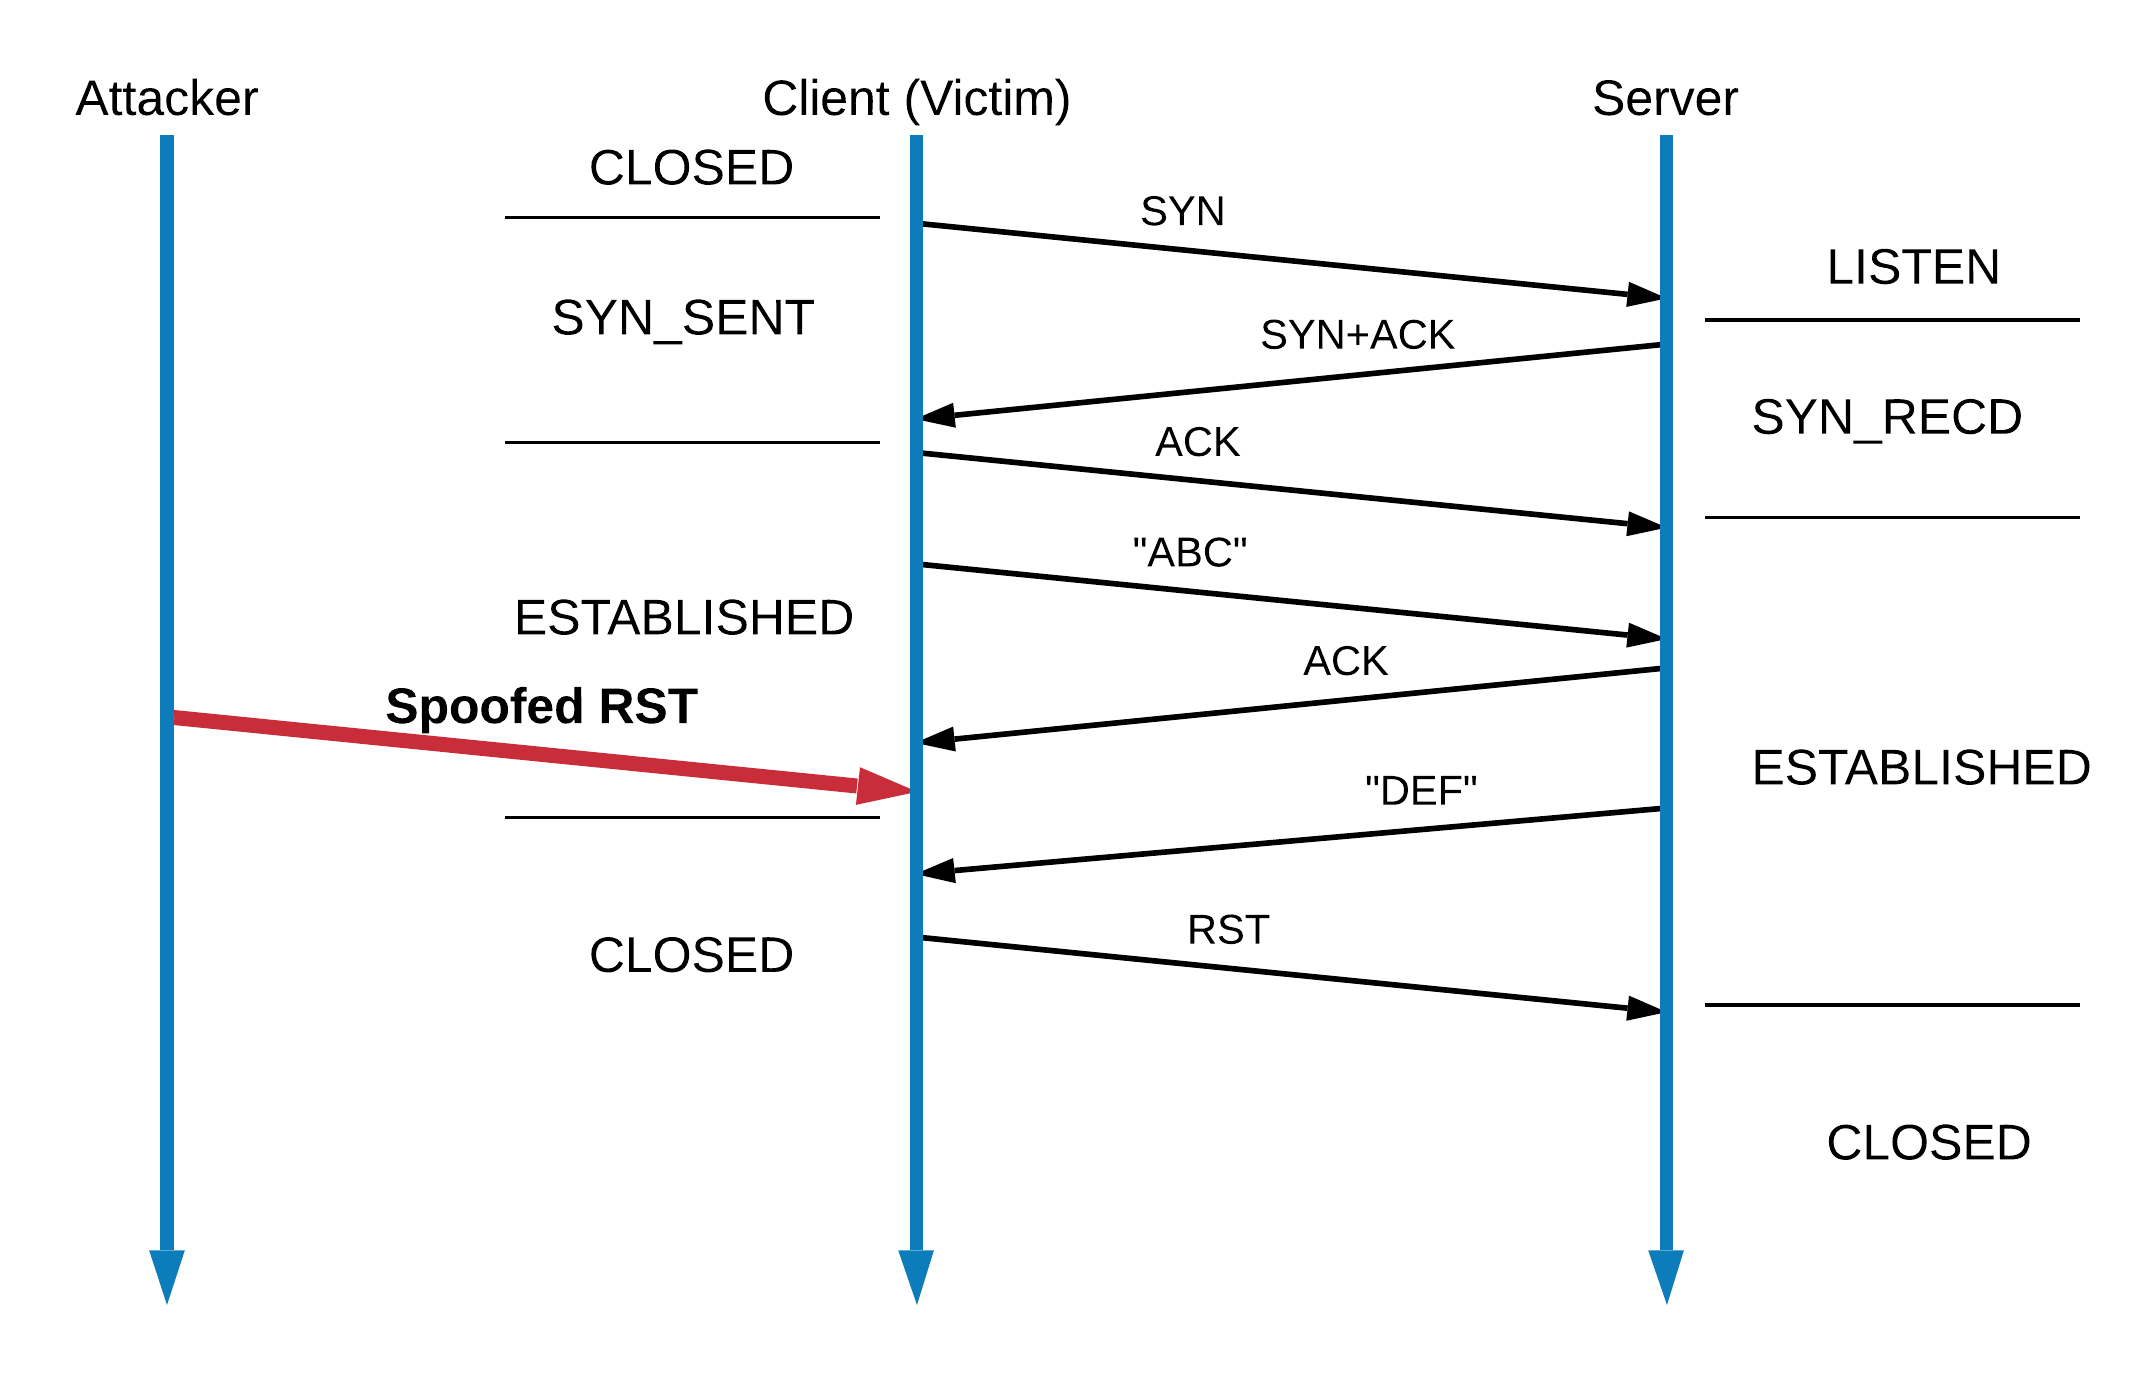
\includegraphics[width=.95\textwidth]{Pictures/Design/TCP_RST_Timing_Diagram.png}
    	\caption{TCP Reset Attack Timing Diagram} 
    	\label{fig:RST_Attack_Tim}
    \end{figure}
    
\section{Packet Details}
    \begin{figure}[!h]
    	\centering
    	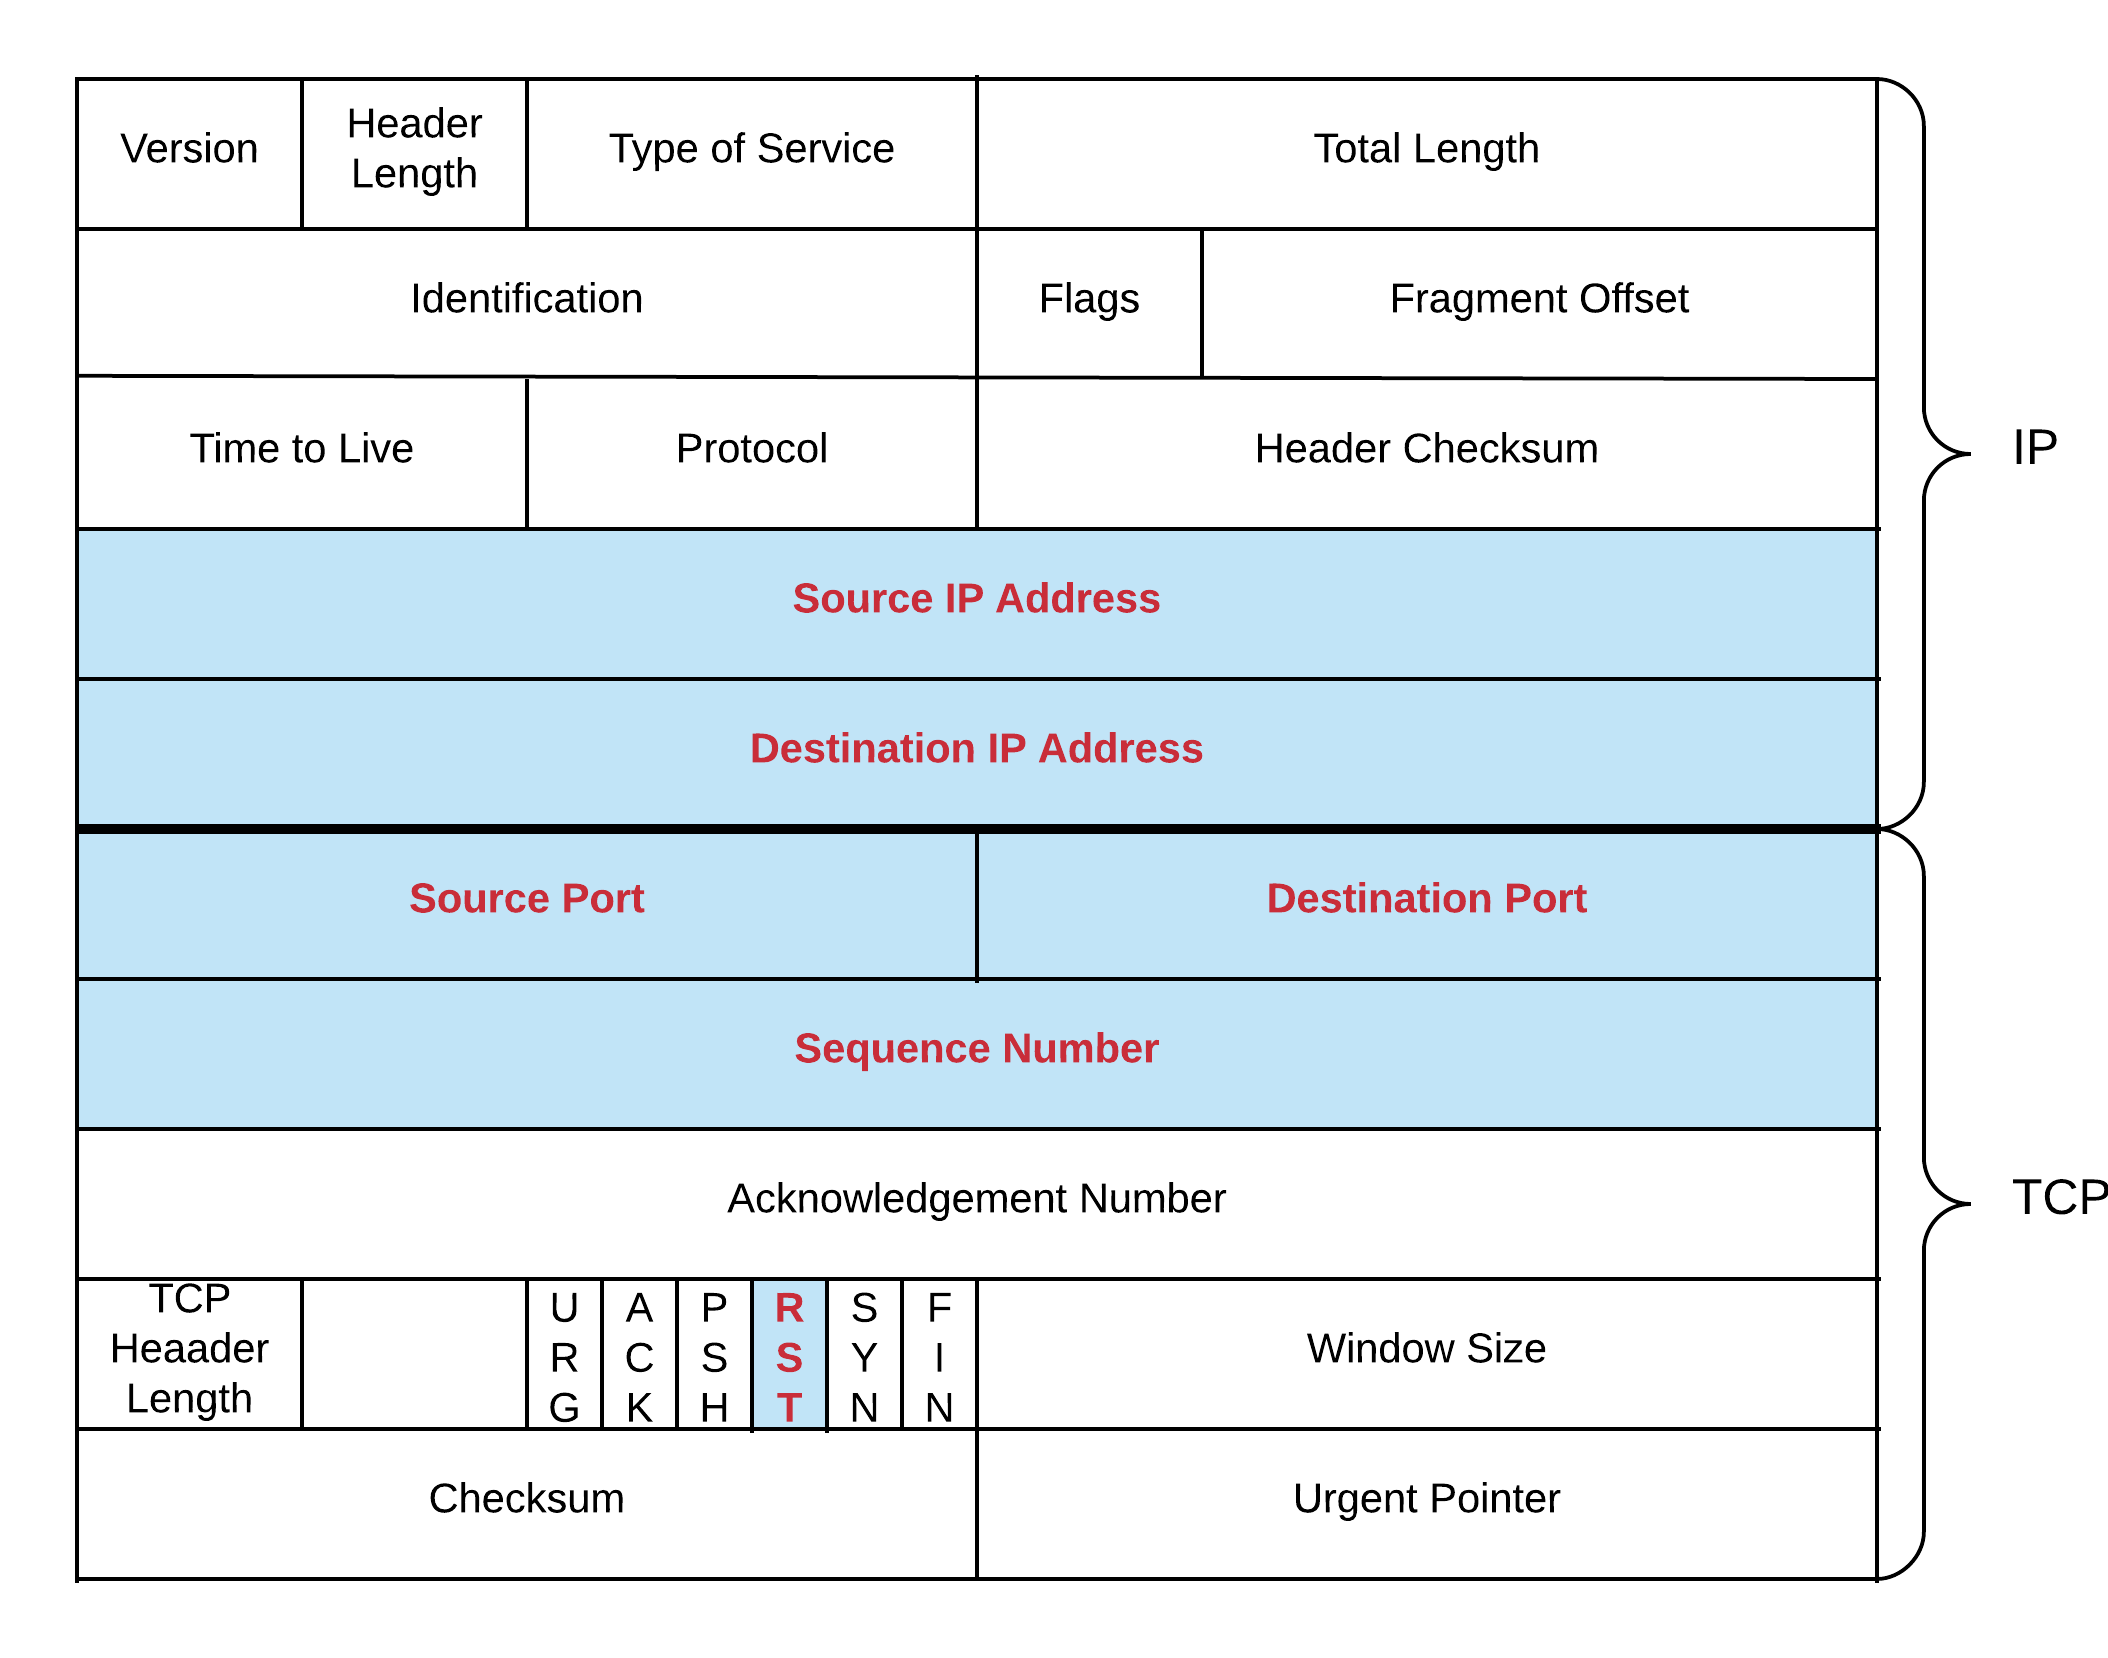
\includegraphics[width=.85\textwidth]{Pictures/Design/TCP_IP_Packet.png}
    	\caption{Attack Packet Header} 
    	\label{fig:Attack_Packet}
    \end{figure}

    In Figure \ref{fig:Attack_Packet}, we show the specific fields in the TCP/IP header that need to be handled in order to perform TCP reset attack. Here source IP will be the video streaming server's IP address, Destination IP will be victim's IP address, and the port numbers will be set correspondingly. Sequence number must be correctly discovered through sniffing. Finally RST bit must be set to 1. The other fields will be set accordingly with the help of programming language libraries. Also payload to this header is not really important in this case as it is merely an RST packet.

\section{Available Tools}
    \label{sec:netwox}
    
    \begin{figure}[!h]
    	\centering
    	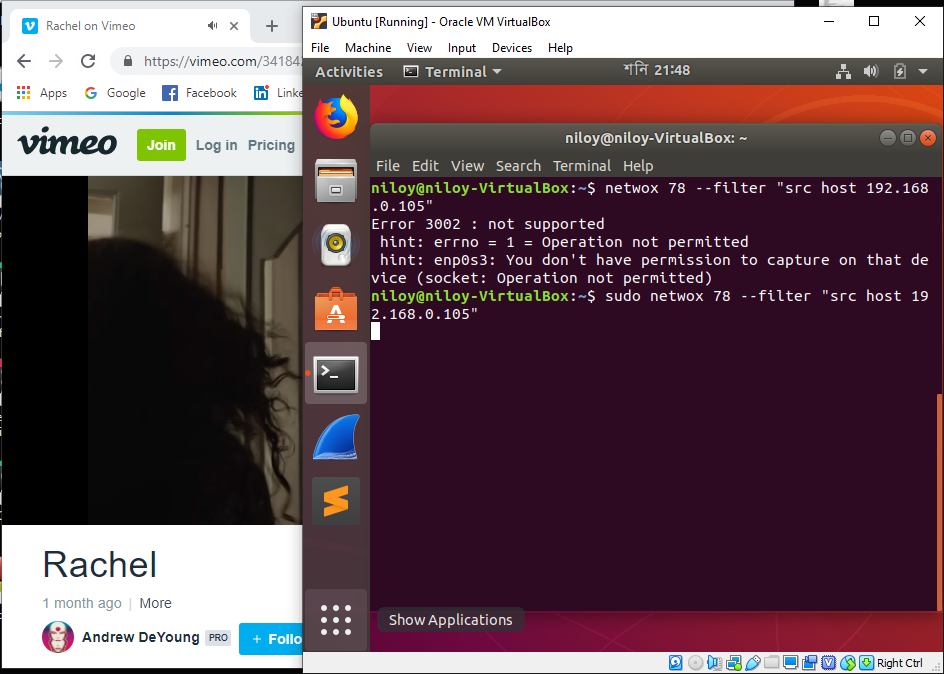
\includegraphics[width=.95\textwidth]{Pictures/Design/Netwox_test.png}
    	\caption{Netwox Test} 
    	\label{fig:netwox_test}
    \end{figure}
    
    There are already a few available tools for many different network attacks. Among them \textbf{Netwox} is a quite well known one. To perform TCP reset attack with Netwox from an Linux environment, the command is as follows:
    
    \subfile{Codes/Netwox.tex}
    
    Although being readily available, there is a major drawback of this Netwox command. For working correctly, we already know from Section \ref{sec:strategy} that sequence number of the forged packet must be within the victims window. Also port numbers must be set correctly. For doing so, sniffing is a must, but it is not possible with "pcap" API for packets from other devices on the network which are connected through switch. As a result where Wireshark does not work, neither does Netwox 78 command. The test with VM environment in Figure \ref{fig:netwox_test} also supports these results discussed above.
    

\section{Implementation Technology}
    \begin{description}
        \item[Programming Language:] We have used \textbf{Python 3.7} for implementation purpose. One of the main reasons for choosing this language is that it has ample support for forging TCP packets and sending them to appropriate destination. 
        
        \item[Libraries:] We need a library to sniff, forge and send packets. In python \textbf{Scapy} is one of the packages which provide support for these tasks. An important reason to choose this package is that it gives us a clean interface which helps us to avoid clumsy socket programming, and consequently makes the implementation simple, easily understandable and portable. We have used Scapy 2.4.0 in this implementation. 
    
    \end{description}
    
    
\section{Implementation Environment}
   \begin{description}
        \item[Operating System:] The scripts have been tested on both Windows 10 and Ubuntu 18.04 as attacker operating system. As victim's operating system, Windows 7 and Windows 10 have been tested.
        
        \item[Networking Technology:] As attacker network interface, only Ethernet has been tested. Attacker connected to WiFi has not been tested with these scripts, but victim can be on the same subnet connected through WiFi.
    
    \end{description}

\section{Implementation Topology}
    \label{sec:implement_topology}
    
    
    We have created a video streaming server in the local network for implementation purpose. In this case the attacker, the server and the victim- all are in the same subnet. So to sniff packets we have to change the mac address table of both the victim and the server, and then we can forge packets accordingly.
    
    In Figure \ref{fig:topolgy_implement}, the video server and the  attacker is connected to the same switch. The victim is connected to a WiFi access point which is then connected to the router. So all of these devices are in the same subnet.
    
    \begin{figure}
    \centering
        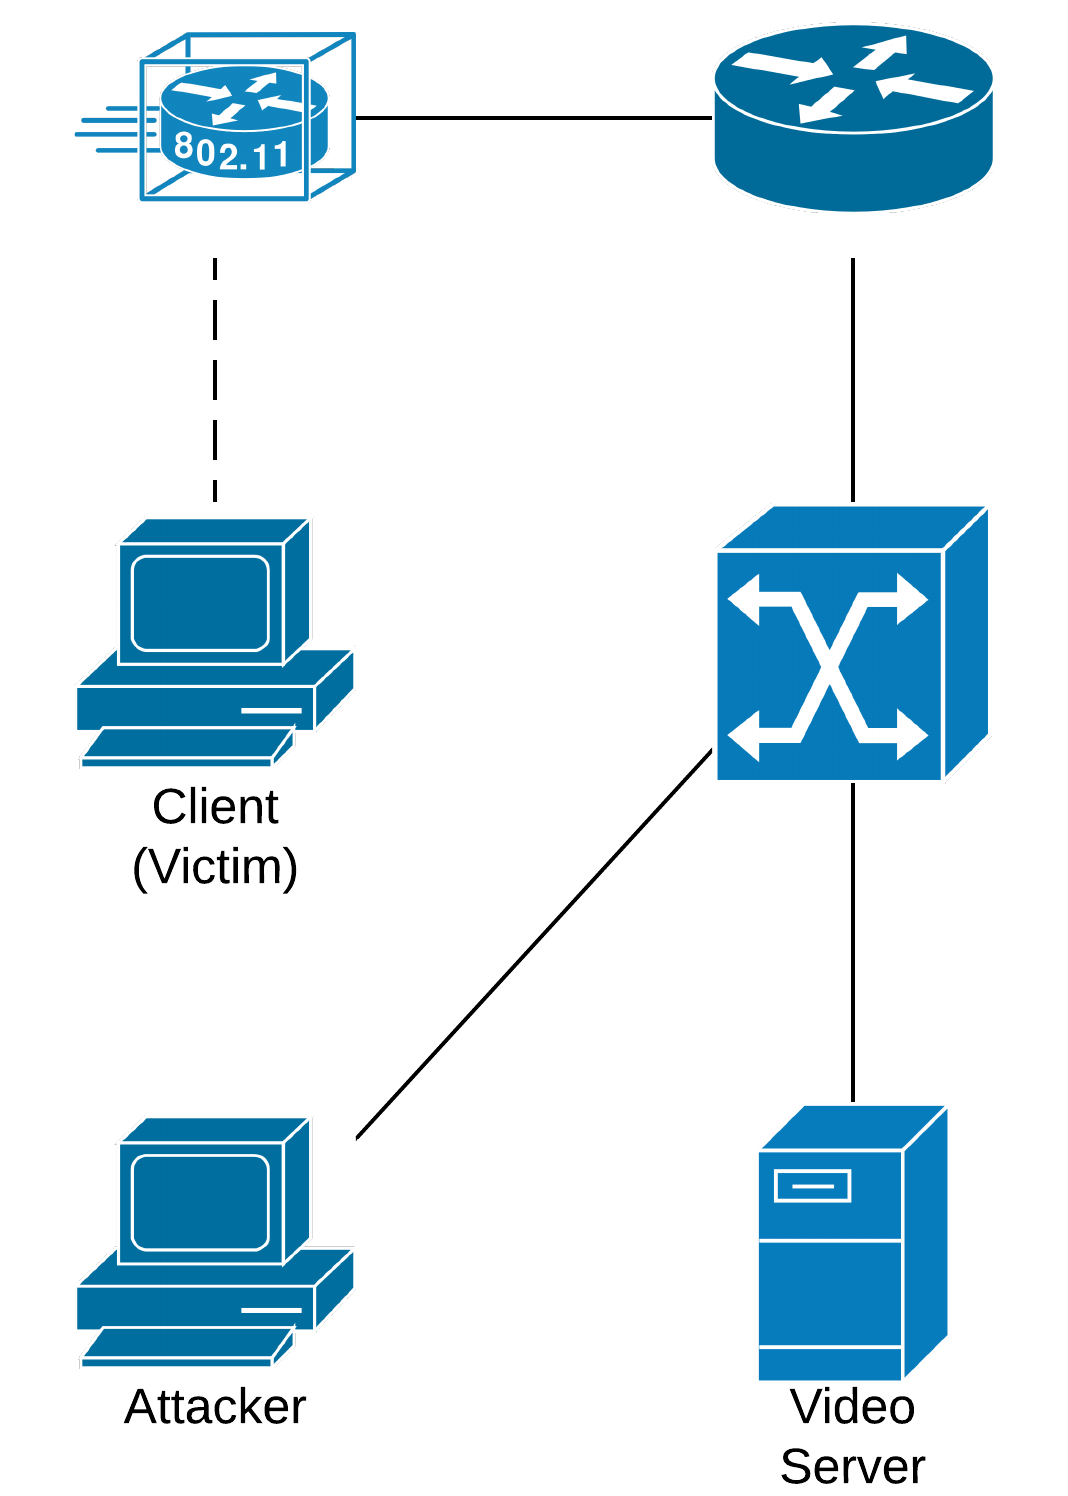
\includegraphics[width=.5\textwidth]{Pictures/Final_TCP_RST_Topology_Implementation.png}
        \caption{Implementation Topology}
        \label{fig:topolgy_implement}
    \end{figure}        
            
            
\section{Testing Topology}
    \label{sec:test_topology}
    \begin{figure}
        \centering
        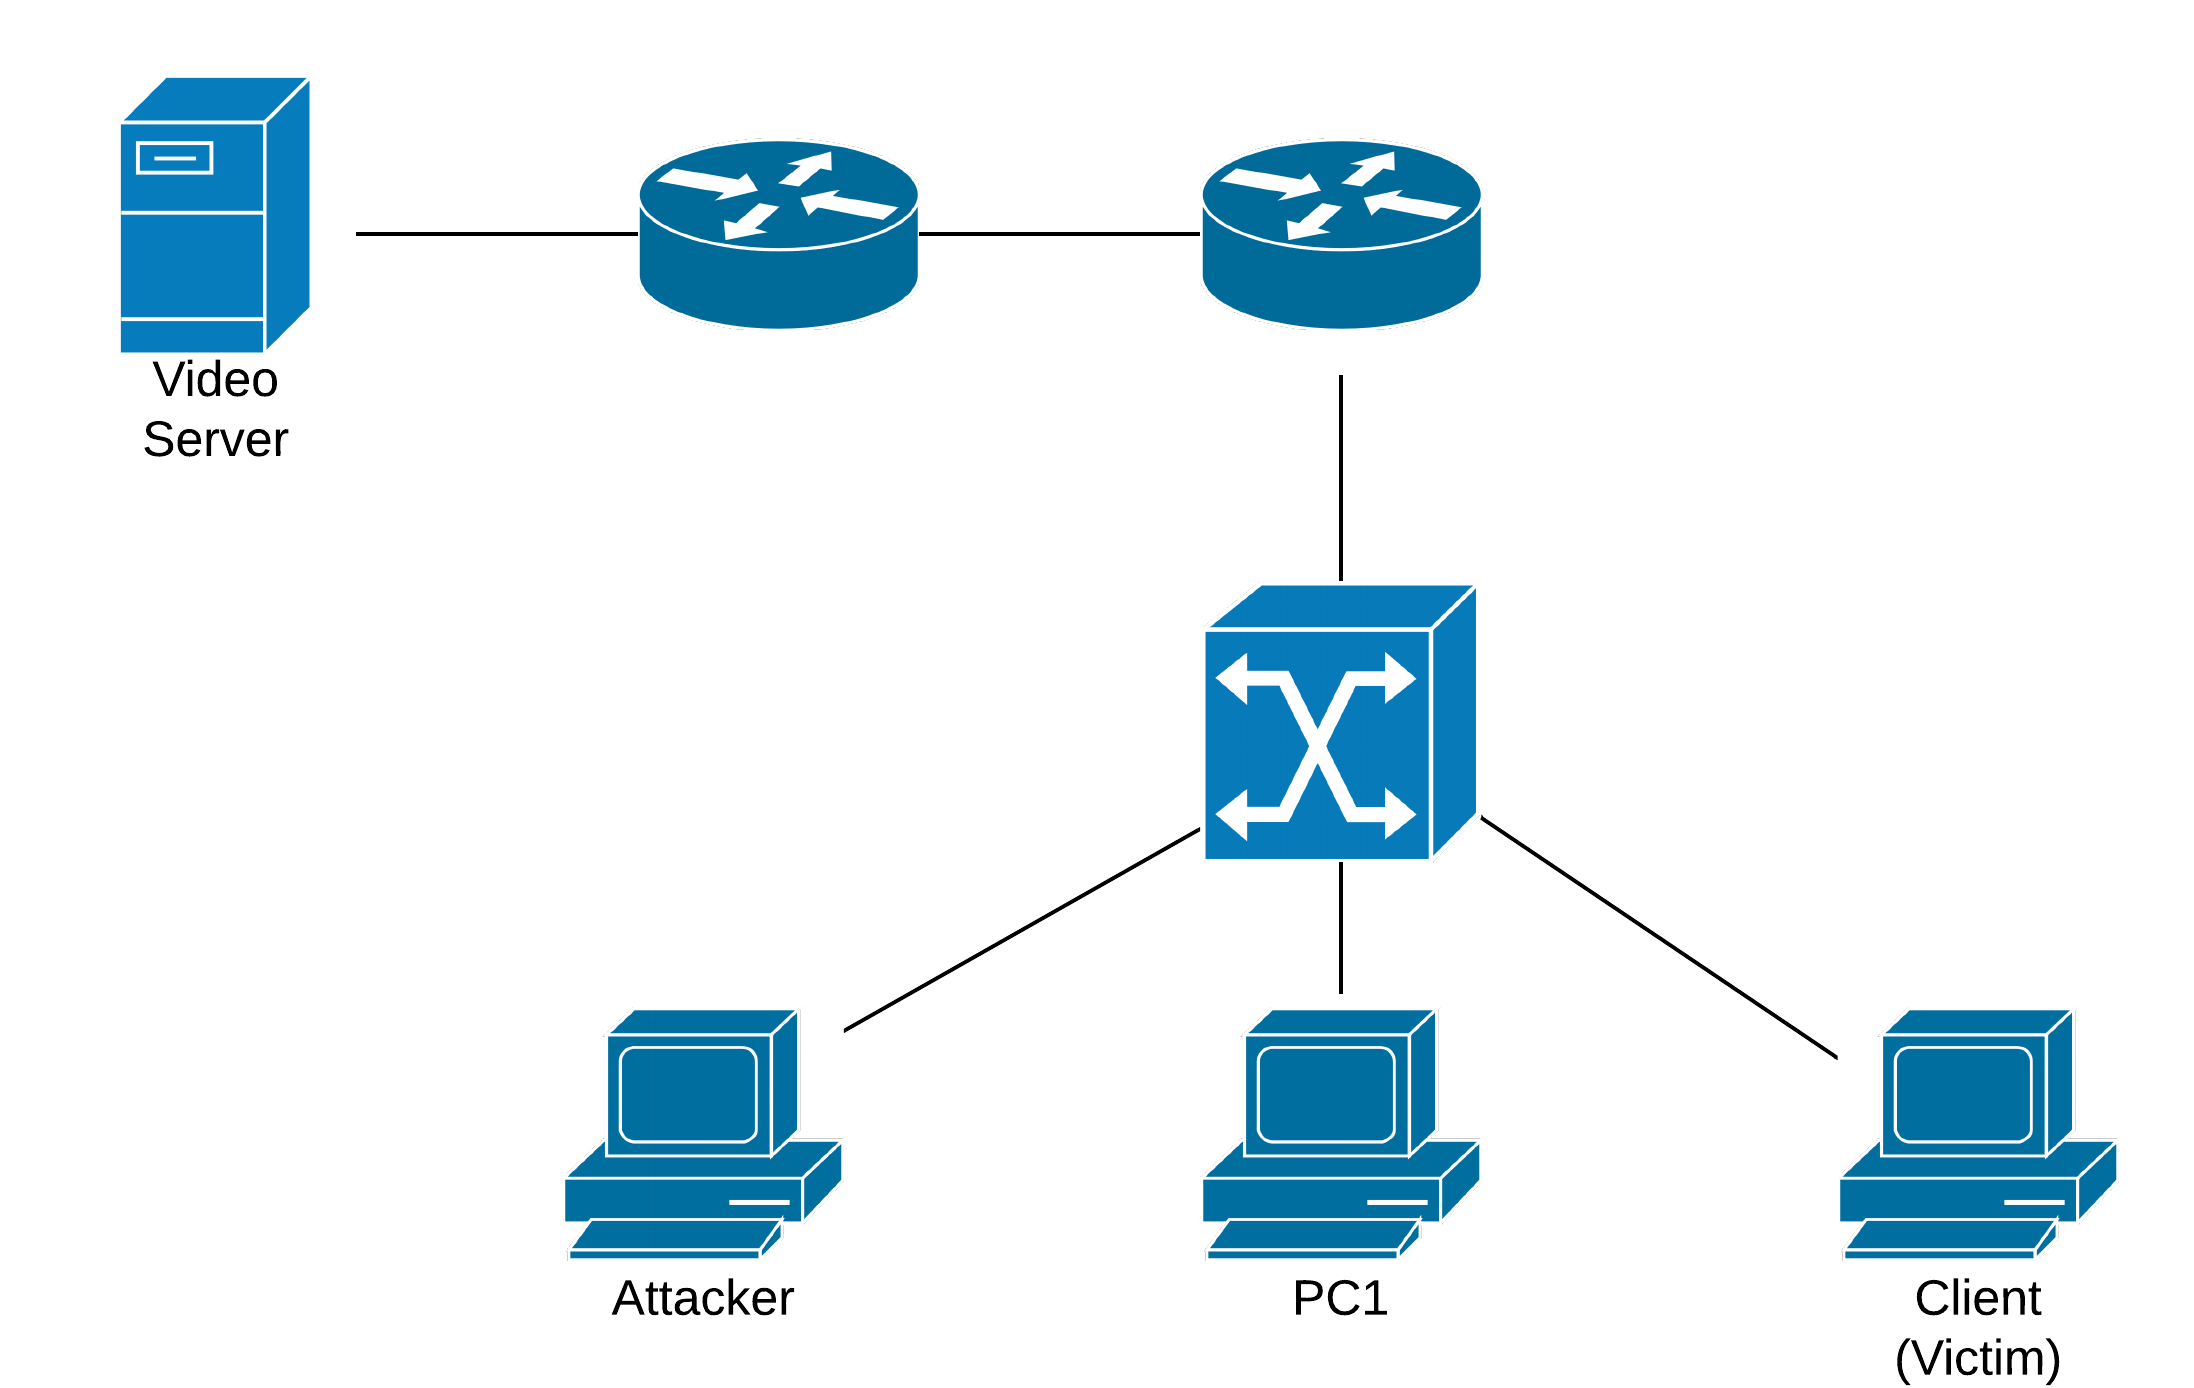
\includegraphics[width=.95\textwidth]{Pictures/Final_TCP_RST_Topology_Test.png}
        \caption{Testing Topology}
        \label{fig:topology}
    \end{figure}
    
     As our testing environment, we have designed a topology as shown in Figure \ref{fig:topology}. Here the attacker and the victim are in the same subnet and the server is in a remote network. Without the loss of generality there can be more switches or routers in the network, and more hosts connected to the switch. This type of topology is carefully chosen as we need to sniff packets destined to the victim machine to gather information about source IP, TCP port numbers and sequence number in order to successfully perform a TCP reset attack.
     
     
     Provided that the tool is a success, it will reach the state of one of a kind because currently available tools cannot work properly, as discussed in Section \ref{sec:netwox}, in such an environment.
    

\section{Implementation Phases}    
    The attack tool is implemented in 2 phases. Those are: 
    \begin{enumerate}
        \item Implementing \textbf{Man-in-the-Middle} (MITM) attack with \textbf{ARP Spoofing} in order to enable the attacker to sniff victim's packets
        \item Implementing \textbf{TCP Reset} attack based on the sniffed packets
    \end{enumerate}
    
    \subsection{Man-in-the-Middle Attack}
        For implementation environment and for testing environment, the Man-in-the-middle attack is slightly different in our case. The contributing factor of this difference is the location of the video streaming server in the network, i.e. whether it is within the same subnet or not. An important note is that to perform this attack without disrupting the entire connection of the victim, we must enable IP forwarding on the attacker's machine.
        
        \subsubsection{For Remote Server}
            For video streaming server outside of subnet, like the one mentioned in Section \ref{sec:test_topology}, we have to sniff packets between the gateway and the victim. For that reason, the following python script is written to change the MAC Address table of those two so that their communication passes through the attacker.
            \subfile{Codes/MITM.tex}
            
            \begin{figure}
                \centering
                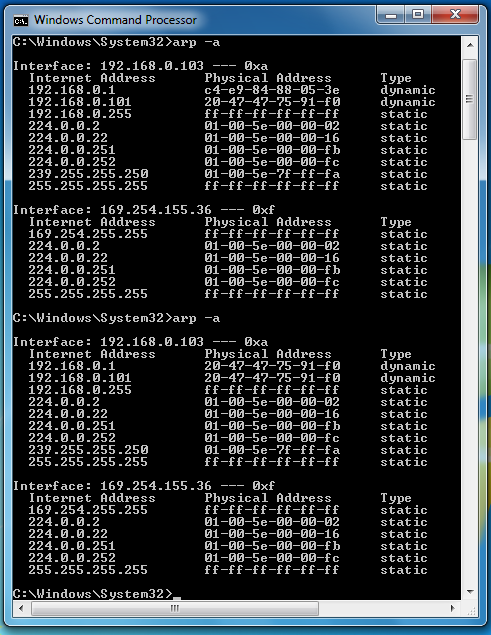
\includegraphics[width=.95\textwidth]{Pictures/MITM_Gateway/arp.png}
                \caption{MAC Address Table of Victim before and after MITM Attack}
                \label{fig:MITM_Gateway_Arp}
            \end{figure}
            
            In the Figure \ref{fig:MITM_Gateway_Arp}, MAC Address table of victim (192.168.0.103) is shown. The important part is that attacker (192.168.0.101) has successfully changed the gateway's (192.168.0.1) MAC address to the one attacker has. The gateway's MAC address table is updated in the same way.
            
            From the perspective of attacker, after running this script, Wireshark can capture packets from the victim (192.168.0.103). This is shown in Figure \ref{fig:MITM_Gateway_Wireshark}.
            
            \begin{figure}
                \centering
                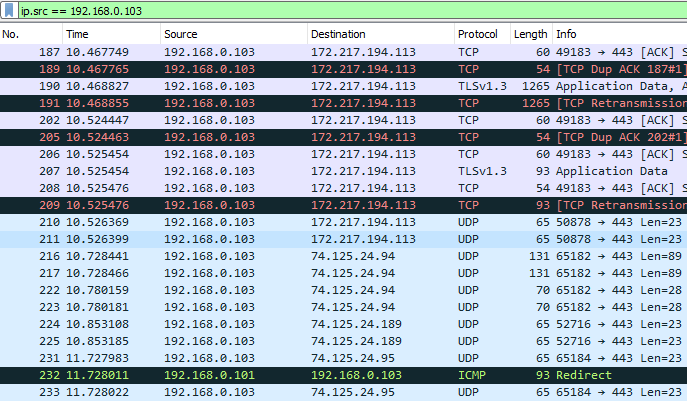
\includegraphics[width=.95\textwidth]{Pictures/MITM_Gateway/AfterMITM_Attacker.png}
                \caption{Wireshark of Attacker after MITM Attack}
                \label{fig:MITM_Gateway_Wireshark}
            \end{figure}
            
        \subsubsection{For Local Server}
             For video streaming server inside the subnet, like the one mentioned in Section \ref{sec:implement_topology}, we have to sniff packets between the server and the victim. For that reason, the following python script is written to change the MAC Address table of those two so that their communication passes through the attacker.
            \subfile{Codes/MITM2.tex}
            
            \begin{figure}
                \centering
                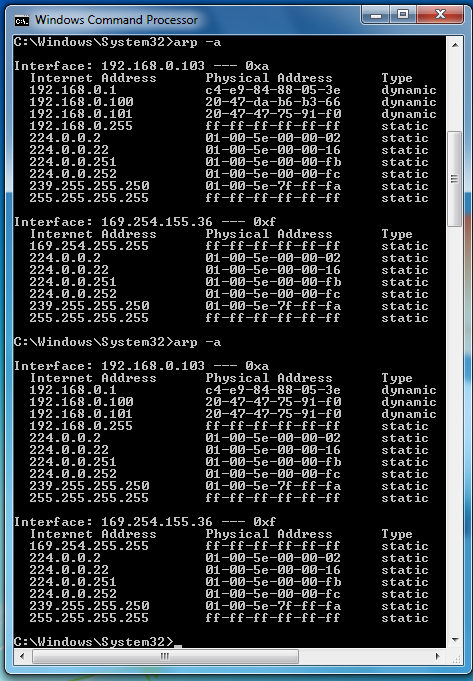
\includegraphics[width=.95\textwidth]{Pictures/MITM_Local/arp.png}
                \caption{MAC Address Table of Server before and after MITM Attack}
                \label{fig:MITM_Local_Arp}
            \end{figure}
            
            In the Figure \ref{fig:MITM_Local_Arp}, MAC Address table of server (192.168.0.103) is shown. In this case, attacker (192.168.0.101) has successfully changed the victim's (192.168.0.100) MAC address to the one attacker has. The victim's MAC address table is updated in the same way.
            
            From the perspective of attacker, after running this script, wireshark can capture packets from the victim (192.168.0.103). This is shown in Figure \ref{fig:MITM_Local_Wireshark}.
            
            \begin{figure}
                \centering
                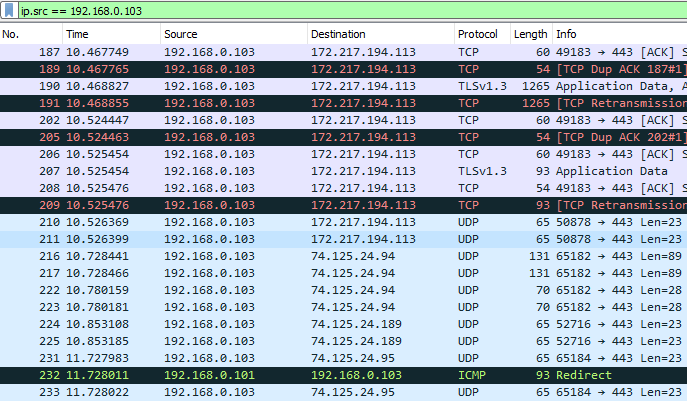
\includegraphics[width=.95\textwidth]{Pictures/MITM_Gateway/AfterMITM_Attacker.png}
                \caption{Wireshark of Attacker After MITM Attack}
                \label{fig:MITM_Local_Wireshark}
            \end{figure}
     
        \subsubsection{Testing MITM's Success}
            \label{sec:sniff}
            In addition to Wireshark, the following script can validate that our Man-in-the-Middle attack is successful. 
            
            \subfile{Codes/Sniffer.tex}
            
            After this successful implementation of Man-in-the-Middle attack, we are ready to go on to implement our actual target - TCP Reset attack.
    
    
    
    \subsection{TCP Reset Attack}
        \label{sec:rst_script}
    
        In this phase we have implemented TCP Reset attack with the help of the sniffing script developed in Section \ref{sec:sniff}. After sniffing, we use the sniffed packets to extract the IP addresses, port numbers and sequence number. The script is as follows:
        
        \subfile{Codes/RST.tex}
        
        Tests on this script is described in the following section.
        
\section{Testing TCP Reset Attack}
    We have tested both on actual websites and on VLC media player stream. Results of these tests are described below.
    
    \subsection{Failed Test: Vimeo}
        Although we have successfully terminated the TCP connection between the victim and Vimeo website, our attack is not being able effectively disrupt video playback. 
        
        \begin{figure}
            \centering
            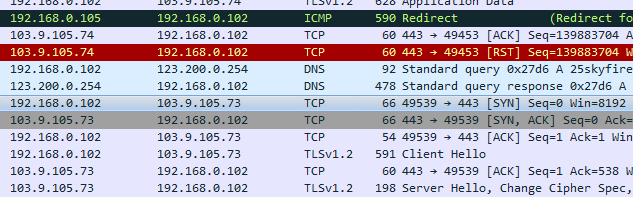
\includegraphics[width=.95\textwidth]{Pictures/Vimeo/Vimeo.png}
            \caption{Test on Vimeo}
            \label{fig:vimeo}
        \end{figure}
        
        As seen in Figure \ref{fig:vimeo}, first the reset packet closes the TCP connection between the victim (192.168.0.102) and the server (103.9.105.74). But the attack eventually failed because the browser of the victim automatically establishes a new connection in the 3-way handshake mechanism using SYN packet with another IP address (103.9.105.73) of the same website. In other words, this website has preventive mechanism against TCP reset attack installed already.
        

    \subsection{Failed Test: Dailymotion}
        Although we have successfully terminated the TCP connection between the victim and Dailymotion website, our attack is not being able effectively disrupt video playback.
        
        \begin{figure}[!h]
            \centering
            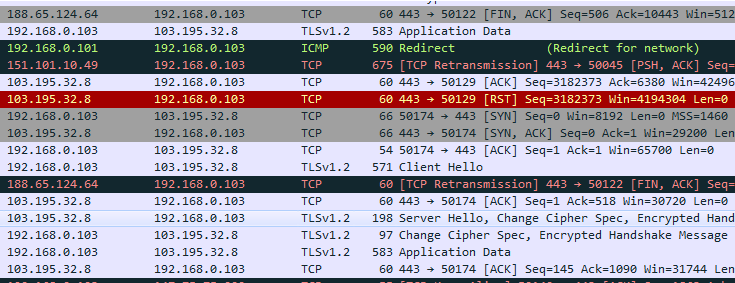
\includegraphics[width=.95\textwidth]{Pictures/Dailymotion/dm.png}
            \caption{Test on Dailymotion}
            \label{fig:dailymotion}
        \end{figure}
        
        As seen in Figure \ref{fig:dailymotion}, first the reset packet closes the TCP connection between the victim (192.168.0.103) and the server (103.195.32.8). But the attack eventually failed because the browser of the victim automatically establishes a new connection in the 3-way handshake mechanism using SYN packet with the same IP address. In other words, this website too has preventive mechanism against TCP reset attack installed already.
        
    \subsection{Successful Test: VLC Stream from Local Server}
        We have created a video streaming server with VLC media player in one of the PCs in the same subnet. It is shown in Figure \ref{fig:before_local} that the victim is viewing from server (192.168.0.103) on 8080 port through WiFi.
        
        \begin{figure}[!h]
            \centering
            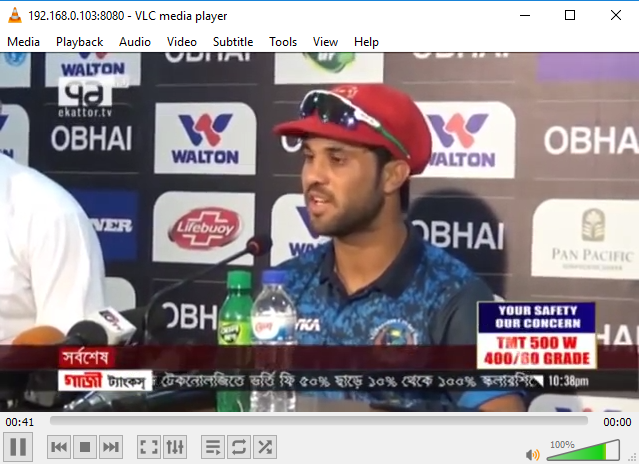
\includegraphics[width=.95\textwidth]{Pictures/RST_Local/before.PNG}
            \caption{Before Attack on VLC Stream from Local Server}
            \label{fig:before_local}
        \end{figure}
        
        After we have started sending RST packets with the script from Section \ref{sec:rst_script}, the video stopped at the victim's VLC player within a short while. This result is shown in Figure \ref{fig:after_local}.
        
        \begin{figure}
            \centering
            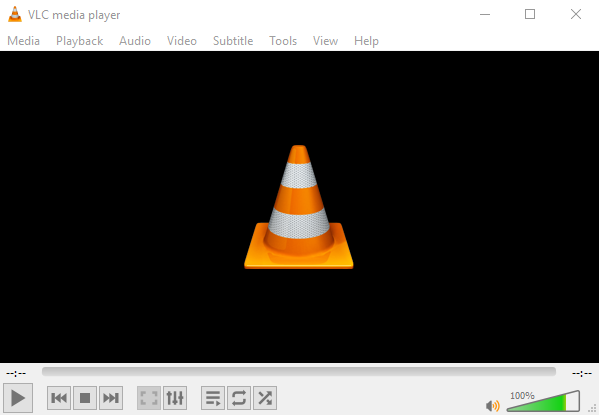
\includegraphics[width=.95\textwidth]{Pictures/RST_Local/after.png}
            \caption{After Attack on VLC Stream from Local Server}
            \label{fig:after_local}
        \end{figure}
        
        
    \newpage
    \subsection{Successful Test: VLC Stream from Remote Server}
        \label{sec:remote_vlc}
        We have created a video streaming server with VLC media player in a PC outside the subnet using TeamViewer. Then we have used \textbf{http tunneling} mechanism with a tool, \textbf{ngrok}, to access that stream. It is shown in Figure \ref{fig:before_remote} that the victim is viewing from server (18.223.41.243) through ngrok tunnel (http://3c88ed6f.ngrok.io) over the internet.
        
        \begin{figure}[!h]
            \centering
            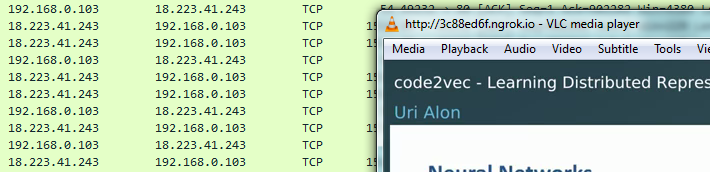
\includegraphics[width=.95\textwidth]{Pictures/RST_Remote/before.png}
            \caption{Before Attack on VLC Stream from Remote Server}
            \label{fig:before_remote}
        \end{figure}
        
        After we have started sending RST packets with the script from Section \ref{sec:rst_script}, the video stopped at the victim's VLC player within a short while. This result is shown in Figure \ref{fig:after_remote}. In this case, we have spoofed a RST packet with source IP address: 18.223.41.243 with correct port numbers and sequence number. As a result the media player has aborted the connection and the video streaming is successfully disrupted.
        
        \begin{figure}
 .        \centering
            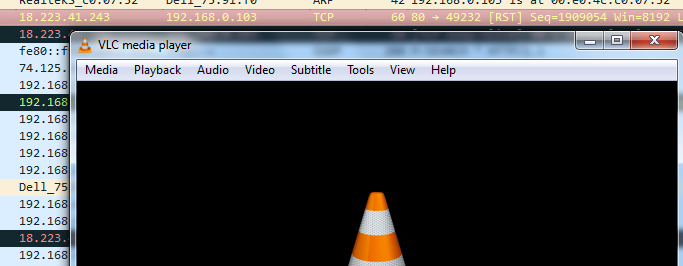
\includegraphics[width=.95\textwidth]{Pictures/RST_Remote/after.png}
            \caption{After Attack on VLC Stream from Remote Server}
            \label{fig:after_remote}
        \end{figure}    


\section{Justification}
    In our implementation we have included both Man-in-the-Middle and TCP reset mechanism. It can be inferred from above discussion that with the help of MITM mechanism, TCP reset can successfully find out correct IP, port numbers and the sequence number, and consequently our tool can exactly mimic a RST packet from the original server. When the victim machine receives the RST packet, it does not have any idea about the packet's actual origin. So the victim machine has no other option but to terminate its TCP connection. 
    
    The test shown in Section \ref{sec:remote_vlc} points out that our approach to TCP reset attack is definitely unique. Currently available tools like netwox fails (shown in Section \ref{sec:netwox}) in the scenario where we have succeeded.

\section{Drawbacks or Future Work}
    \begin{enumerate}
        \item Although we have succeeded in disrupting video streams in some case, our tools fails to achieve any considerable impact on modern websites with preventive measures. 
        
        \item Tests have been performed on only Windows as Operating System of the victim. Other operating systems including Ubuntu, Mac OS needs to be tested. Also Mac OS as attacker's operating system should also be tested.
        
        \item Our scripts have been written based on the assumption that the attacker is connected with the subnet through Ethernet technology, not with WiFi. Attack with connected through WiFi is also needed to be developed and tested.
    
    \end{enumerate}
    


\section{Defence Mechanism}
    A defense mechanism for our attack tool can easily be derived from the above design. A simple time delay can effectively disable the effect of our attack. It is described below:
    
    \begin{enumerate}
        \item Whenever we receive an RST packet from video streaming server, we add a time delay before closing the connection rather than doing so immediately.
        \item If we receive additional packets from the server within the time delay with correct sequence numbers, we can assume the RST packet was actually a spoofed one.
        \item Otherwise after the time delay, we close the connection in the same way as it would normally do.
    \end{enumerate}
    
    Here this defense mechanism should work properly because the original server is likely to retransmit the packets that were lost due too ARP spoofing and upon receiving the actual packets the victim can take appropriate measure.
    
\section{Conclusion}
    We have discussed different aspects of the implementation of an attack tool to exploit a particular vulnerability of TCP. Nevertheless it is an inseparable part of today's internet. So as our concluding remarks, we hope that this attack tool may in turn provide us the insight about how to defend against such attacks.
    

\section{Repository}
    The scripts and documentation can be viewed in the following repository: 
    \verb!https://github.com/ishtiaqniloy/TCP_Reset_Attack_Video_Streaming! \\
    Scripts can be found in \verb!"Python_Implementation"! folder. \\
    Full sized screenshots can be found in \verb!"Documentation/Screenshot"! folder.

\section{References}
    \begin{enumerate}
        \item https://tools.ietf.org/html/rfc793
        \item https://en.wikipedia.org/wiki/Transmission\_Control\_Protocol
        \item https://en.wikipedia.org/wiki/TCP\_reset\_attack
        \item https://en.wikipedia.org/wiki/Man-in-the-middle\_attack
        \item http://www.cis.syr.edu/~wedu/seed/Book/book\_sample\_tcp.pdf
        \item https://medium.com/secjuice/man-in-the-middle-attack-using-arp-spoofing-fa13af4f4633
        \item https://null-byte.wonderhowto.com/how-to/build-man-middle-tool-with-scapy-and-python-0163525/
        \item https://scapy.readthedocs.io/en/latest/usage.html
        \item https://www.howtogeek.com/118075/how-to-stream-videos-and-music-over-the-network-using-vlc/
        \item https://ngrok.com/docs
    \end{enumerate}


\end{document}
